\section{FrameWork}
Since refactoring tools to correcly transform the program often require the same information about the program, such as
the AST and the def-use-relations, they often have similar architecture.
This similarity between refactoring tools creates the possibility of reusing some modules
instead of creating every module from scratch which makes refactoring tools
development a lot faster.
Creating a framework for refactoring tools increases both the speed and the simplicity (??)
of creating a refactoring tool. In addition the framework is able to reuse the features already available
for one refactoring tool in the others without extra effort. Such features highly improve
the usefulness of a refactoring tool, for example the highlight of possible refactoring
operations, the previewing of the result and support to detect duplicated code.

%Refactoring static languages
As we do not explore type information to do refactoring operations to static typified
programing languages we can not say that we do refactoring for static languages.
However, there are fragments/subsets of those languages that may be refactored by our
framework. Those fragments are parts of the code that can be reason upon without using
the type information, for example:

Ideally we should only have refactoring operations for the meta-language which represents
all the implemented languages combined with specialized pretty printers to output the changes in the
desireble language.
However, such general representation would be complex and would also reduce the languages
expressiveness.
Instead of having a general representation that can represent all the languages
supported we have the languages represented in syntax objects representative of the language.

In addition, we also have a meta-language that abstracts all the supported languages and
we have trully language independent refactoring operations. However, it is only
for a small set of refactoring opeartions, the simpler ones.
And since we have a restrict amount of time, having
a meta-language that have language-independent refactoring operations combined
with the syntax-objects representation which have similar refactoring operations but
language dependent and therefore more specialized.

%[TODO Explain META-LANGUAGE]
We decided to implement the framework in Racket since it were already some programming
languages implmented languages for DrRacket which made the development of the framework easier.

With this combination we do not have a language-independent framework. However we have a framework
for refactoring dynamic languages.
Framework architecture.%FIXME this is super weird
\begin{figure}[h]
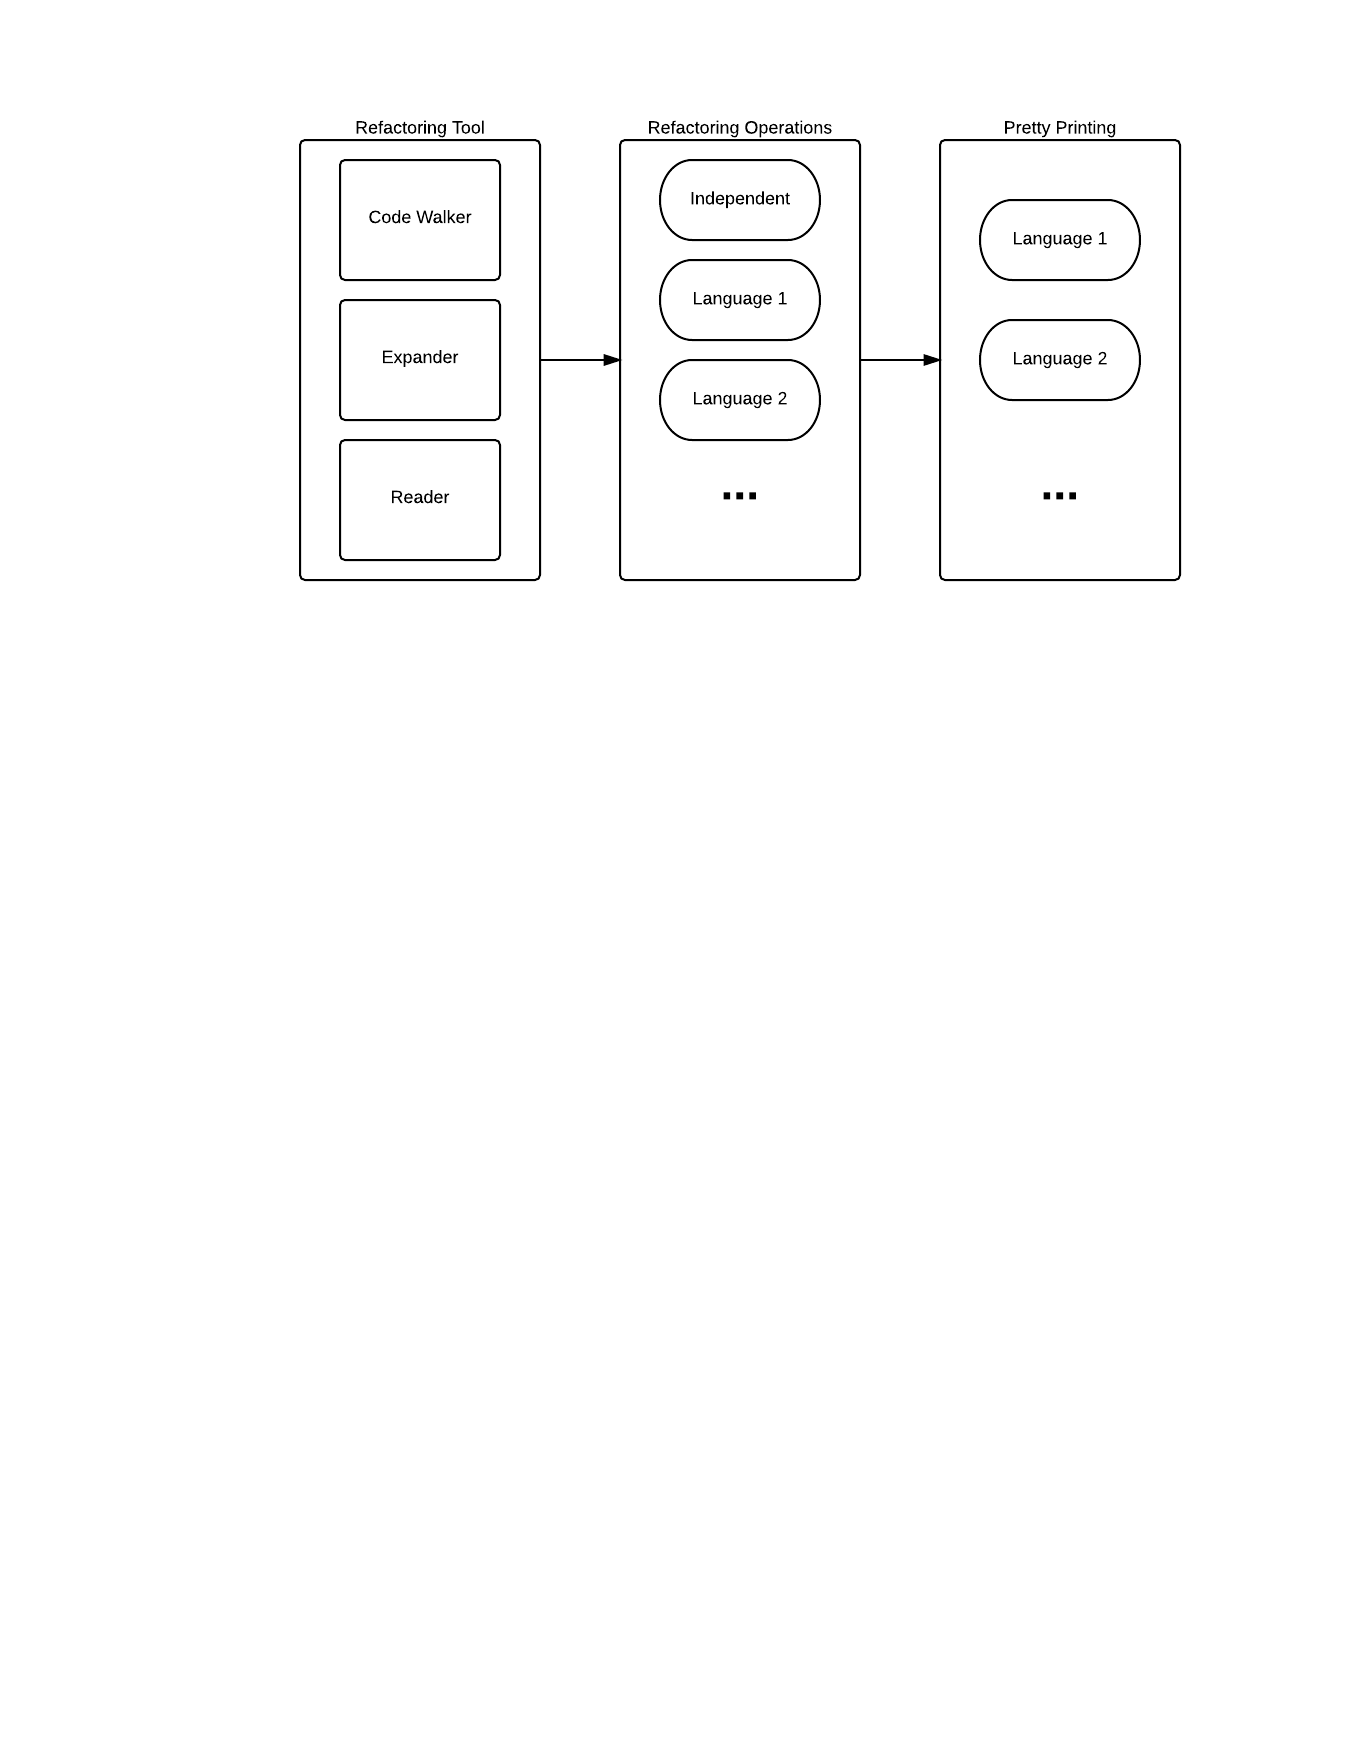
\includegraphics[width=8cm]{../framework-arch2.png}
\label{fig:framework}
\end{figure}

As it is described in Figure~\ref{fig:framework} we have a module that provides
independent refactoring operations and a module for each language supported that
have specialized refactoring operations. We also have pretty-printing modules for
each supported language.

We already have refactoring operations for Racket, Python, and Processing. We choose
this languages since they are already implemented in Racket and they are often used by beginners.


\subsection{Statement based languages}
This Framework was build with a base of expression based languages. The flow of
the program is needed to decide whether or not a refactoring can be correctly done
or even to decide where and how many returns a function needs. However this could
be minimized with a PDG (program depedence graph) that has the control flow information
needed to compute correct refactorings.

\subsection{Language Independent refactoring operations}
Creating a fully language independent refactoring tool is difficult since programming
languages differ semantically from each other, even some operations that are semantically
equal for most of the cases, for the cases that they are not semantically equal makes it very
difficult to do a general refactoring operation.
%TODO give an example. (+ in python?) (< ?)
However, for simple refactoring opeartions, which do not require much program semantics,
it is possible to have language independente refactoring operations in a meta-language that
represents the semanatic of the other implemented languages. %TODO CHECK THIS

\subsection{Language dependent refactoring operations}
It is necessary to have refactoring operations that are language dependent, since
some refactoring operatons have particular cases for each supported language.
Having specific refactoring operations, language dependent ones, it is possible
to implement some useful refactoring operations in a simple way that otherwise would
be too complex.
%TODO give an example

\section{Features} %talk about one feature fits all
%how easy it is to add new refactoring operations and languages
One important part of this framework is to seamsly provide the features created
having in mind one refactoring tool to every refactoring tool developed within this
framework.
This is possible because the refactoring tools use the same information represented
in the form of syntax objects. The syntax-objects have several information regarding
location and position that can be used.
For example it is possible to use the highlight of the possible refactoring operations
in the several languages.

%Automatic detection
%Preview
%duplicated code detection
\section{Requirements?Goals}
The framework it is simply to use, it is only necessary to have a specification file
of each refactoring operation.
That file must have a function that receives two arguments,
one is the AST of the program and the other is the def-use-relation.
This information makes it possible to have several refactoring operations that help
the programmer.
%what was "reused"
%everything except the refactoring operations itself.
%the advantages of that
This Framework makes it easier to implement refactoring operations for dynamic languages,
with only the catch that they have to be implemented for DrRacket. Helping minimizing
the problem of the difficulty and lacking of refactoring operations for dynamic languages.
(for at least every language implemented for DrRacket)




\subsection{Interoperability} %interoperability?

IDEs are always evolving and DrRacket is no execption. Therefore developing a refactoring tool
inside the editor itself is not a good idea. The solution to cope with all the future changes
is to create a plugin. This plugin ensures that for the vast majority of modifications in DrRacket
our refactoring tool will be able to work properly without any modification.
The plugin itself also makes it easier to port the refactoring tool to another editor.
Another advantage of the plugin relies on how DrRacket manages the plugins. If the plugin
is deployed in a git repository any commits made to that repository will trigger
a reinstalation from DrRacket therefore providing the most updated version of the refactoring tool.

\section{Tool Maintenance} %Framework maintenance!
%Developer Point of view
A refactoring tool is a quite complex piece of software and therefore requires maintenance.
Automatic testing is used in general by developers to ensure that the software
is bug free for those test cases.
Automatically testing all the refactoring operations is a good way to test if
the changes inserted any bugs in the refactoring tool.
One way to automatic test the refactoring operations is to apply every refactoring
operations possible in a piece of code. By having such possibility it is simpler
to the developer to create specific test cases simplifying tool maintenance.
In order to do this it is necessary to correctly identify all the possible refactoring
operations in one piece of code, which is already implemented in the refactoring
tool, and apply all of refactoring operations found.
Since every refactoring operation changes the AST which changes the position of the
lines of code and it also may change the possible refactoring operations it is necesasry to recompute the
program AST before the next iteration of the algorithm.


\section{Examples}  %evaluation?
%examples in python:
%examples in processing:

\subsection{Translator}
Using the meta-language capabilities it is even possible to translate code
from one language to another.

Example: Python -> Racket -> Processing
%TODO insert example:
\section{Analysis} %and conclusion
Combining the two approaches can simply create refactoring operations for several
languages targetted at beginner programmers. Some of this refactoring operations
are rather simple, when compared to more advanced ones, and some can even be reproduced
in a meta-language and therefore only implemented once for several programming languages.
For the rest of the refactoring operations they can be added to the dependent language
module in which it is possible to have the special cases covered.

With the combination usage of reader + expander + code-walker working for the several
implemented languages most of the work is already done and when combined with the
powerfulness offered by the syntax-parser it is possible to create refactoring operations
using only one line of code, e.g. %TODO add an example
Even having some refactoring operations that are more complex it is way quicker and
simpler only to have to implement the refactoring operation itself.
However, there is still lacking of program information that is rather useful for
statement based languages (or even object oriented ones?) which is program dependence.
%extract function for python + processing, atm is kinda tricky!
Having more program information available, such as the dependence, it is possible to
create even more complex refactoring operations which would be a great improvement.


%\section{Conclusion}

\section{Future Work}
Add a PDG to the framework. and other forms of representing the program information.
Simplify even further adding languages to the framework
Simplify even further create features for all languages.
Create an API??
